\section*{ÔN TẬP CHƯƠNG I}
\setcounter{ex}{0}\setcounter{bt}{0}
\Opensolutionfile{ans}[ans/ans-KTTX-1-2]

\begin{ex}%[0K1Y1-3]
Phủ định của mệnh đề \lq\lq  $\exists x\in \mathbb{R}:2x^2-3x-5<0$\rq\rq\  là
\choice
{ \True \lq\lq  $\forall x\in \mathbb{R}:2x^2+3x-5\ge 0$ \rq\rq }
{\lq\lq  $\forall x\in \mathbb{R}:2x^2+3x-5>0$\rq\rq }
{\lq\lq  $\exists x\in \mathbb{R}:2x^2+3x-5>0$\rq\rq}
{ \lq\lq $\exists x\in \mathbb{R}:2x^2+3x-5\ge 0$\rq\rq }
\loigiai{Phủ định của mệnh đề \lq\lq  $\exists x\in \mathbb{R}:2x^2-3x-5<0$\rq\rq\  là mệnh đề \lq\lq  $\forall x\in \mathbb{R}:2x^2+3x-5\ge 0$ \rq\rq.
}
\end{ex}

\begin{ex}%[0K1Y1-3]%[0-GK1-NH22-23--TeamTeXHoa--Sơn Bùi]
Mệnh đề phủ định của $P\colon$\lq\lq $\forall x \in \mathbb{R}, x^{2}>0$\rq\rq\,  là
\choice
{$\bar{P}\colon$\lq\lq $\forall x \in \mathbb{R}, x^{2} \leq 0$\rq\rq}
{\True $\bar{P}\colon$\lq\lq $\exists x \in \mathbb{R}, x^{2} \leq 0$\rq\rq}
{$\bar{P}\colon$\lq\lq $\exists x \in \mathbb{R}, x^{2}< 0$\rq\rq}
{$\bar{P}\colon$\lq\lq $\forall x \in \mathbb{R}, x^{2}< 0$\rq\rq}
\loigiai{Mệnh đề $P\colon$\lq\lq $\forall x \in \mathbb{R}, x^{2}>0$\rq\rq, phủ định của mệnh đề $P$ là $\bar{P}\colon$\lq\lq $\exists x \in \mathbb{R}, x^{2} \leq 0$\rq\rq.}
\end{ex}

\begin{ex}%[0-GK1-NH22-23--TeamTeXHoa--Don Lee]%[0K1Y1-1]
Trong các câu sau có bao nhiêu câu là mệnh đề toán học?
\begin{listEX}[2]
\item[] $(1)$: Số $3$ là số chẵn.
\item[] $(2)$: $2x+1=3$.
\item[] $(3)$: Các em hãy cố gắng làm bài thi tốt.
\item[] $(4)$: $1<3 \Rightarrow 4<2$.
\end{listEX}
\choice
{\True $2$}
{$3$}
{$1$}
{$4$}
\loigiai{
"Số $3$ là số chẵn là mệnh đề." và "$1<3 \Rightarrow 4<2$."
}
\end{ex}

\begin{ex}%[0K1Y2-1]
\immini{
Cho  $ A, $ $ B $   là hai tập hợp bất kì. Phần gạch sọc trong hình vẽ bên dưới là tập hợp nào sau đây?
}{
\begin{tikzpicture}[scale=0.4]
\def\firstven{(0,0) ellipse (3cm and 2cm)}
\def\secondven{(3.2,0) ellipse (3cm and 2cm)}
\begin{scope}
\clip \firstven;
\fill[pattern=north east lines,opacity=1] \secondven;
\end{scope}
\draw \firstven \secondven;
\node at (-1,0) {$A$};
\node at (3.8,0){$B$};
%			\node at (3.5,-1.7){$A \cap B$};
\end{tikzpicture}
}
\choice
{ $B\backslash A$ }
{\True $A \cap B$ }
{  $A\backslash B$}
{ $A \cup B$ }
\loigiai{
}
\end{ex}

\begin{ex}%[0K1Y2-1]
Liệt kê các phần tử của tập hợp $A=\big\{ x \in \mathbb{N} \mid x<5\big\}$.
\choice
{$A=\big\{1;2;3;4;5\big\}$}
{$A=\big\{1;2;3;4\big\}$}
{$A=\big\{0;1;2;3;4;5\big\}$}
{\True $A=\big\{0;1;2;3;4\big\}$}
\loigiai{
$A=\big\{ x \in \mathbb{N} \mid x<5\big\}=\big\{0;1;2;3;4\big\}$.
}
\end{ex}

\begin{ex}%[0K1Y2-2]
Cho tập hợp $A=\big\{1;2;3\big\}$. Tập hợp nào sau đây \textbf{không} là tập con của tập $A$?
\choice
{$\big\{1;2;3\big\}$}
{$\big\{1;2\big\}$}
{$\varnothing$}
{\True $\big\{1;3;4\big\}$}
\loigiai{
Tập hợp $\big\{1;3;4\big\}$ \textbf{không} là tập con của tập hợp $A$ vì có $4 \notin A$.
}
\end{ex}

\begin{ex}%[0K1Y1-4]%[0K1Y1-4]%[0K1Y1-4]
Mệnh đề đảo của mệnh đề $P\Rightarrow Q$ là mệnh đề nào?
\choice
{\True $Q\Rightarrow P$}
{$Q\Rightarrow\overline{P}$}
{$Q\Rightarrow\overline{P}$}
{$\overline{Q}\Rightarrow P$}
\loigiai{
Mệnh đề đảo của mệnh đề $P\Rightarrow Q$ là mệnh đề $Q\Rightarrow P$.
}
\end{ex}

\begin{ex}%[0K1Y2-4]
Tập hợp nào sau đây chỉ gồm các số vô tỷ?
\choice
{$\mathbb{Q} \setminus \mathbb{N}^*$}
{\True $\mathbb{R} \setminus \mathbb{Q}$}
{$\mathbb{Q} \setminus \mathbb{Z}$}
{$\mathbb{R} \setminus \big\{0\big\}$}
\loigiai{
Tập hợp chỉ gồm các số vô tỷ là $\mathbb{R} \setminus \mathbb{Q}$.
}
\end{ex}

\begin{ex} %[0K1Y2-1]
Cho hai tập hợp $X = \left\{ { - 1\,;\,2\,;\,4\,;\,7\,;\,9} \right\}$  và $Y = \left\{ { - 1\,;\,0\,;\,7\,;\,10} \right\}$  . Tập hợp $X \cap Y$  có bao
nhiêu phần tử?
\choice
{ $ 3 $ }
{ $ 7 $ }
{\True $ 2 $ }
{ $ 5 $ }
\loigiai{$ X\cap Y= \{-1;7\} $ có 2 phần tử.
}
\end{ex}

\begin{ex}%[0K1Y1-2]
Với giá trị nào của  $x$ thì $x^2-1=0, x \in \mathbb{N}$    là mệnh đề đúng?
\choice
{\True $x=1$ }
{$x=\pm 1$ }
{ $x=-1$}
{ $x=0$}
\loigiai{ Ta có  $x^2-1=0\Leftrightarrow \hoac{&x=1 \in \mathbb{N}\\&x=-1 \notin \mathbb{N}.}$
}
\end{ex}

\begin{ex}%[0K1Y1-3]
Phủ định của mệnh đề \lq \lq$\forall x\in \mathbb{R},{{x}^{2}}-x+7<0$\rq\rq \ là
\choice
{\True \lq \lq $\exists x\in \mathbb{R}, \ x^2-x+7\ge 0$\rq\rq }
{\lq \lq$\forall x\in \mathbb{R},\ x^2-x+7>0$\rq\rq }
{\lq \lq$\forall x\in \mathbb{R},\ x^2-x+7<0$\rq\rq }
{\lq \lq$ \exists x\in \mathbb{R},\ x^2-x+7<0$\rq\rq }
\loigiai{ Phủ định của mệnh đề \lq \lq$\forall x\in \mathbb{R},{{x}^{2}}-x+7<0$\rq\rq \ là mệnh đề
\lq \lq $\exists x\in \mathbb{R}, \ x^2-x+7\ge 0$\rq\rq
}
\end{ex}

\begin{ex}%[0K1Y1-3]
Tìm mệnh đề phủ định của mệnh đề sau:  $ \forall x\in\mathbb{N}, x^2-1\geq 0 $.
\choice
{$ \forall x\in\mathbb{N}, x^2-1\leq 0 $}
{$ \forall x\in\mathbb{N}, x^2-1>0 $}
{$ \exists x\in\mathbb{N}, x^2-1\geq 0 $}
{\True $ \exists x\in\mathbb{N}, x^2-1<0 $}
\loigiai{
Phủ định của mệnh đề  $ \forall x\in\mathbb{N}, x^2-1\geq 0 $ là   $ \exists x\in\mathbb{N}, x^2-1<0 $.
}
\end{ex}

\begin{ex}%[0K1Y1-2]
Cho phương trình bậc hai $ ax^2+bx+c=0 $ với $ a\neq 0 $ . Mệnh đề nào dưới đây sai?
\choice
{Phương trình trên vô nghiệm khi và chỉ khi  $ \Delta <0 $}
{Phương trình trên có hai nghiệm trái dấu khi và chỉ khi  $ \dfrac{c}{a}<0 $}
{Phương trình trên có nghiệm khi và chỉ khi  $ \Delta \geq 0 $}
{\True Phương trình trên có hai nghiệm âm phân biệt khi và chỉ khi  $ ac>0 $}
\loigiai{
Xét phương trình bậc hai  $ ax^2+bx+c=0$.
\begin{itemize}
\item  Phương trình trên vô nghiệm khi và chỉ khi  $ \Delta <0 $ là một mệnh đề đúng.
\item  Phương trình trên có hai nghiệm trái dấu khi và chỉ khi $ \dfrac{c}{a}<0 $  là một mệnh đề đúng.
\item  Phương trình trên có nghiệm khi và chỉ khi  $ \Delta \geq 0 $ là một mệnh đề đúng.
\item  Phương trình trên có hai nghiệm âm phân biệt khi và chỉ khi $ ac>0 $  là một mệnh đề sai.
Phương trình có hai nghiệm âm phân biệt $ \Rightarrow ac>0 $  là một mệnh đề đúng.\\
Phương trình có $ ac>0 $  thì phương trình có hai nghiệm âm phân biệt là một mệnh đề sai. Chẳng hạn như xét phương trình  $ x^2-3x+2=0 $ có $ ac=2>0 $  nhưng lại có hai nghiệm dương phân biệt là  $ x=1 $ và  $ x=2 $.
Do đó phương trình có hai nghiệm âm phân biệt khi và chỉ khi $ ac>0 $  là một mệnh đề sai.
\end{itemize}
}
\end{ex}

\begin{ex}%[0K1B1-2]
Phát biểu nào sau đây là một mệnh đề \textbf{sai}?
\choice
{ $\exists x \in \mathbb{Z},\,\,x + 1 = 0$ }
{\True $\forall x \in \mathbb{R},\,\,\left| {x - 1} \right| - x + 1 > 0$}
{  $\forall x \in \mathbb{R},\,\,{x^2} \ge 0$}
{ $\exists x \in \mathbb{Q},\,\,2{x^2} - 3x + 1 \ne 0$}
\loigiai{
Xét mệnh đề \lq\lq  $\forall x \in \mathbb{R},\,\,\left| {x - 1} \right| - x + 1 > 0$\rq\rq là một mệnh đề với mọi.\\
Chọn $ x=1: |x - 1|\, - x + 1=0>0 $ là sai. Do đó, mệnh đề sai.
}
\end{ex}

\begin{ex}%[0K1B2-1]
Cho tập hợp $A=\left\{ \left. x\in \mathbb{N} \right|\left( 2x+6 \right)\left( x-3 \right)=0 \right\}$. Số phần tử của tập hợp $A$ là
\choice
{ $0$}
{\True $1$}
{ $3$}
{ $2$}
\loigiai{
Ta có $\left( 2x+6 \right)\left( x-3 \right)=0\Leftrightarrow \left[ \begin{aligned}
& 2x+6=0 \\
& x-3=0 \\
\end{aligned} \right.\Leftrightarrow \left[ \begin{aligned}
& x=-3\notin \mathbb{N} \\
& x=3\in \mathbb{N}. \\
\end{aligned} \right.$\\
Vậy $A=\left\{ 3 \right\}$ nên tập $A$ có 1 phần tử.}
\end{ex}

\begin{ex}%[0-GK1-NH22-23--TeamTeXHoa--Hồng Trường Sơn]%[0K1B2-1]
Trong các tập hợp sau, tập hợp nào là tập hợp rỗng?
\choice
{\True $A= \left\{ x \in \mathbb{R} \mid x^2+2x+3=0 \right\}$}
{$C= \left\{ x \in \mathbb{R} \mid x^2-3=0 \right\}$}
{$B= \left\{ x \in \mathbb{R} \mid x^2-4=0 \right\}$}
{$D= \left\{ x \in \mathbb{R} \mid x^2+x-12=0 \right\}$}
\loigiai{
Ta có phương trình $x^2+2x+3=0$ vô nghiệm.\\
Do đó $A = \varnothing$.
}
\end{ex}

\begin{ex}%[0-GK1-NH22-23--TeamTeXHoa--NguyenTruongVinh]%[0K1B2-2]
Cho hai tập hợp $ X_1=\left\lbrace x \in \mathbb{R}|(x-2)(x-1)=0\right\rbrace  $ và $ X_2=\left\lbrace x \in \mathbb{R}|x(x^2-4)(x^2-1)=0\right\rbrace  $. Khẳng định nào sau đây đúng?
\choice
{\True $ X_1 \subset X_2 $}
{$ X_1 =X_2$}
{$ X_1 \cap X_2=\varnothing $}
{$ X_2 \subset X_1$}
\loigiai{
Ta có $ (x-2)(x-1)=0 \Leftrightarrow \hoac{&x=2 \in \mathbb{R}\\&x=1 \in \mathbb{R}}\Rightarrow X_1=\left\lbrace 1;2\right\rbrace  $.\\
$ x(x^2-4)(x^2-1)=0\Leftrightarrow \hoac{&x=0\in \mathbb{R}\\&x=\pm 2 \in \mathbb{R}\\&x=\pm 1 \in \mathbb{R}}\Rightarrow X_2 =\left\lbrace -2;-1;0;1;2\right\rbrace $.\\
Vậy $ X_1\subset X_2 $.

}
\end{ex}

\begin{ex}%[0K1B1-2]
Mệnh đề chứa biến  $P:\forall x \in \mathbb{R},\,\,{x^2} - 2 + a > 0$ với $ a $ là một số thực cho trước. Tìm tất cả các số thực $ a $  để  $ P $ đúng.
\choice
{ $a \le 2$ }
{$a < 2$  }
{ $a = 2$ }
{\True $a > 2$ }
\loigiai{
Điều kiện $ -2+a>0\Leftrightarrow a>2. $
}
\end{ex}

\begin{ex} %[0K1B2-3]
Gọi ${A}$ là tập hợp các hình thoi, ${B}$ là tập hợp các hình chữ nhật và ${C}$ là tập hợp các hình vuông. Mệnh đề nào sau đây đúng?
\choice
{ \True $A\cap B=C $}
{ $A\backslash B=C$}
{ $B\backslash A=C$}
{ ${A\cup B=C}$
}
\loigiai{
Ta có hình thoi có hai cạnh kề vuông góc khi và chỉ khi nó là hình vuông.\\
Hình chữ nhật có hai cạnh kề bằng nhau khi và chỉ khi nó là hình vuông.\\
Vậy $A\cap B=C $.

}
\end{ex}

\begin{ex}%[0K1B1-3]
Cho mệnh đề \lq\lq $\forall x \in \mathbb{R} ,\,\,{x^2} - x + 7 < 0$ \rq\rq. Mệnh đề phủ định của mệnh đề trên là
\choice
{\True $\exists \,x \in \mathbb{R}, {x^2} - x + 7 \ge 0$ }
{ $\forall x \in \mathbb{R},\,\,{x^2} - x + 7 > 0$ }
{ $\forall x \in \mathbb{R},\,\,{x^2} - x + 7 < 0$ }
{ $\exists \,x \in \mathbb{R} ,\,\,{x^2} - x + 7 < 0$ }
\loigiai{ Mệnh đề phủ định là $\exists \,x \in \mathbb{R}, {x^2} - x + 7 \ge 0$.
}
\end{ex}

\begin{ex} %[0K1B2-3]
Cho các tập hợp $M=[ 1;\,4 ]$, $N = (2; 6)$ và $P=( 1;\,2 )$. Tìm tập hợp $(M \cap N) \cap P$.
\choice
{ $[0; 4]$}
{ $[5; + \infty )$}
{ $(- \infty; 1)$}
{ \True $\varnothing $}
\loigiai{
Ta có $M\cap N=(2;4]\Rightarrow M\cap N\cap P=(2;4]\cap (1;2)=\varnothing.$}
\end{ex}

\begin{ex}%[0K1B1-2]
Trong các mệnh đề tương đương sau, mệnh đề nào là mệnh đề {\bf{sai}}?
\choice
{Một tứ giác là hình vuông khi và chỉ khi tứ giác đó là hình thoi và có $ 1 $  góc vuông}
{Một tam giác là tam giác vuông khi và chỉ khi tam giác đó có số đo $ 1 $ góc bằng tổng số đo $ 2 $ góc còn lại}
{\True Hai tam giác bằng nhau khi và chỉ khi chúng đồng dạng và có $ 1 $ góc bằng nhau}
{Một tam giác là tam giác đều khi và chỉ khi nó có $ 2 $ cạnh bằng nhau và có $ 1 $ góc có số đo bằng $ 60^\circ $}
\loigiai{
\begin{itemize}
\item 	\lq\lq  Một tứ giác là hình vuông khi và chỉ khi tứ giác đó là hình thoi và có $ 1 $  góc vuông\rq\rq đúng vì Tứ giác  $ ABCD $ là hình vuông $ \Leftrightarrow $  tứ giác $ ABCD $  có $ 4 $  cạnh bằng nhau và có $ 4 $  góc vuông $ \Leftrightarrow $  tứ giác  $ ABCD $ là hình thoi và có  $ 1 $ góc vuông.
\item \lq\lq  Một tam giác là tam giác vuông khi và chỉ khi tam giác đó có số đo $ 1 $ góc bằng tổng số đo $ 2 $ góc còn lại\rq\rq\, đúng vì giả sử $ \widehat{A} = \widehat{B}+ \widehat{C}\Leftrightarrow  2\widehat{A}=180^\circ\Leftrightarrow  \widehat{A}=90^\circ\Leftrightarrow \triangle ABC$ vuông tại $ A $.
\item \lq\lq  Hai tam giác bằng nhau khi và chỉ khi chúng đồng dạng và có $ 1 $ góc bằng nhau\rq\rq\, sai vì khi hai tam giác đồng dạng thì sẽ có $3$ góc bằng nhau nhưng hai tam giác chưa chắc bằng nhau.
\item \lq\lq  Một tam giác là tam giác đều khi và chỉ khi nó có $ 2 $ cạnh bằng nhau và có $ 1 $ góc có số đo bằng $ 60^\circ $\rq\rq\, đúng vì tam giác có $2$ cạnh bằng nhau và có $1$ góc có số đo là  $ 60^\circ\Leftrightarrow $   tam giác cân có $1$ góc có số đo là $ 60^\circ\Leftrightarrow $  tam giác đó là tam giác đều.
\end{itemize}
}
\end{ex}

\begin{ex}%[0-GK1-NH22-23--TeamTeXHoa--Hồng Trường Sơn]%[0K1B1-3]
Phủ định của mệnh đề \lq\lq  $\forall x \in \mathbb{R}, x + \dfrac{1}{x} \ge 2$\rq\rq \, là mệnh đề
\choice
{\lq\lq  $\exists  x \in \mathbb{R}, x + \dfrac{1}{x} > 2$\rq\rq}
{\lq\lq  $\exists x \in \mathbb{R}, x + \dfrac{1}{x} \ne 2$\rq\rq}
{\lq\lq  $\exists x \in \mathbb{R}, x + \dfrac{1}{x} \le 2$\rq\rq}
{\True \lq\lq  $\exists x \in \mathbb{R}, x + \dfrac{1}{x} < 2$\rq\rq}
\loigiai{
Phủ định của mệnh đề \lq\lq  $\forall x \in \mathbb{R}, x + \dfrac{1}{x} \ge 2$\rq\rq \, là mệnh đề \lq\lq  $\exists x \in \mathbb{R}, x + \dfrac{1}{x} < 2$\rq\rq.
}
\end{ex}

\begin{ex}%[0-GK1-NH22-23--TeamTeXHoa--Hồng Trường Sơn]%[0K1B2-7]
Cho hai tập hợp $A= \left[1;4\right)$ và $B= \left[2;8\right]$. Tìm $A \setminus B$.
\choice
{$A \setminus B = \left[2;4\right)$}
{$A \setminus B = \left[4;8\right]$}
{$A \setminus B = \left[1;8\right]$}
{\True $A \setminus B = \left[1;2\right)$}
\loigiai{
\begin{center}
\tikz{
\draw[-stealth] (0,0)--(8,0);
\path (2,0) node{$\big[$} +(90:0.4) node{$1$}--(5,0) node{$\big)$} +(90:.4) node{$4$};
\fill[pattern=north east lines] (0,-4pt) rectangle (2,4pt) (5,-4pt) rectangle (8,4pt);

\draw[-stealth] (0,-1)--(8,-1);
\path (3,-1) node{$\big[$} +(90:0.4) node{$2$}--(6,-1) node{$\big]$} +(90:.4) node{$8$};
\fill[pattern=north east lines] (0,-1.15) rectangle (3,-0.85) (6,-1.15) rectangle (8,-0.85);

\draw[-stealth] (0,-2)--(8,-2);
\path (2,-2) node{$\big[$} +(90:0.4) node{$1$}--(3,-2) node{$\big)$} +(90:.4) node{$2$};
\fill[pattern=north east lines] (0,-2.15) rectangle (2,-1.85) (3,-2.15) rectangle (8,-1.85);
\draw (-1,0) node {$A$} (-1,-1) node {$B$} (-1,-2) node {$A \setminus B$};
%\draw[-stealth] (3,-.1)--(3,-.6) node[below]{$[a;b]$};
}
\end{center}
Ta có $A \setminus B = \left[1;2\right)$.
}
\end{ex}

\begin{ex} %[0K1B1-4]
Cho  hai mệnh đề
${P}$: \lq\lq  Tuần này tôi mua một vé xổ số Vietlott\rq\rq, và
${Q}$: \lq\lq  Tôi trúng ${100}$ tỉ đồng\rq\rq.\\
Mệnh đề nào dưới đây {\bf không phải} là mệnh đề ${P \Leftrightarrow Q}$?
\choice
{ Tuần này tôi mua một vé xổ số Vietlott nếu và chỉ nếu tôi trúng ${100}$ tỉ đồng}
{ Tuần này tôi mua một vé xổ số Vietlott khi và chỉ khi tôi trúng ${100}$ tỉ đồng}
{ \True Nếu tuần này tôi mua một vé xổ số Vietlott thì tôi trúng ${100}$ tỉ đồng}
{ Tuần này tôi mua một vé xổ số Vietlott là điều kiện cần và đủ để tôi trúng ${100}$ tỉ đồng.
}
\loigiai{
Mệnh đề	\lq\lq  Nếu tuần này tôi mua một vé xổ số Vietlott thì tôi trúng ${100}$ tỉ đồng\rq\rq \  không phải là mệnh đề $P \Leftrightarrow Q$.
}
\end{ex}

\begin{ex}%[0K1B2-1]
Cho tập hợp $A=\left\{x \in \mathbb{N}^* \mid 2 x^2-7 x+3=0 \text{ hoặc } x^3-8 x^2+15 x=0\right\}$, $A$ được viết theo kiểu liệt kê là
\choice
{$A=\{0 ; 5 ; 3\}$}
{\True $A=\{5 ; 3\}$}
{$A=\left\{0 ; \dfrac{1}{2}; 5 ; 3\right\}$}
{$A=\{3\}$}
\loigiai{
Ta có
\begin{itemize}
\item  $2 x^2-7 x+3=0 \Leftrightarrow\hoac{&x=3 \\ &x=\dfrac{1}{2}}.$
\item $x^3-8 x^2+15 x=0 \Leftrightarrow x\left(x^2-8 x+15\right)=0 \Leftrightarrow\hoac{
& x = 0   \\
& x ^ { 2 } - 8 x + 1 5 = 0 }
\Leftrightarrow \hoac{&	x=0 \\
&x=5 \\
&x=3.}$
\end{itemize}
Kết hợp với điều kiện $x \in \mathbb{N}^*$ ta được tập hợp $A$ viết theo kiểu liệt kê các phần tử là: $A=\{3 ; 5\}$.
}
\end{ex}


\begin{ex} %[0K1K2-3]
Cho hai tập $A=\left\{ x\in \mathbb{Z}: \  \dfrac{2x-1}{x+3}\in \mathbb{Z}  \right\}$ và $B=\left\{ 4;\,6;\,8;\,10 \right\}$. Tập hợp $A\cup B$ bằng
\choice
{ $\left\{ 4 \right\}$}
{ $\left\{ 4;\,6;\,8;\,10 \right\}$}
{ $\left\{ -4;\,-10;\,4;\,6;\,8 \right\}$}
{ \True $\left\{ -2;\,-4;\,-10;\,4;\,6;\,8;\,10 \right\}$}
\loigiai{
Ta có $\dfrac{2x-1}{x+3}=2-\dfrac{7}{x+3}\in \mathbb{Z}$. Mà $x \in \mathbb{Z} $ nên suy ra $\dfrac{7}{x+3}\in \mathbb{Z}$ hay
\[\hoac{&x+3=1\\&x+3=-1\\&x+3=7\\&x+3=-7}\Leftrightarrow \hoac{&x=-2\\&x=-4\\&x=4\\&x=-10.}\]
Do đó $A= \left\{-10;-4;-2;4\right\}$. Ta có $B=\left\{ 4;\,6;\,8;\,10 \right\}$.\\
Do đó $A\cup B= \left\{ -2;\,-4;\,-10;\,4;\,6;\,8;\,10 \right\}$.
}
\end{ex}

\begin{ex}%[0K1K2-3]%[0-GK1-NH22-23--TeamTeXHoa--Sơn Bùi]
Cho tập hợp $A=\left(-\infty ; m^2\right)$ và $B=(16 ;+\infty)$. Tập hợp các giá trị thực của $m$ để $A \cap B \neq \varnothing$ là
\choice
{\True $(-\infty ;-4) \cup(4 ;+\infty)$}
{$(-4 ; 4)$}
{$(-\infty ;-4] \cup[4 ;+\infty)$}
{$[-4 ; 4]$}
\loigiai{Để $A \cap B \neq \varnothing \Leftrightarrow m^{2}>16 \Rightarrow m \in(-\infty ;-4) \cup(4 ;+\infty)$.}
\end{ex}

\begin{ex}%[0K1K2-6]
Cho khoảng $A=\left( 1;m+7 \right)$ và nửa khoảng $B=\left[ 2m+3;13 \right)$ ($m$ là tham số). Gọi $S$ là tập hợp tất cả các số nguyên $m$ sao cho $A\cup B=\left( 1;13 \right)$. Tổng các phần tử của tập hợp $S$ là
\choice
{\True $10$}
{ $9$}
{ $-5$}
{ $21$}
\loigiai{
Điều kiện đối với $m$ để tồn tại khoảng $A$ và nửa khoảng $B$ là \[\left\{ \begin{aligned}
& m+7>1 \\
& 2m+3<13 \\
\end{aligned} \right.\Leftrightarrow -6<m<5. \left( * \right)\]
Khi đó
\[A\cup B=\left( 1\,;\,13 \right)\Leftrightarrow \left\{ \begin{aligned}
& 2m+3>1 \\
& 2m+3\le m+7 \\
& m+7\le 13 \\
\end{aligned} \right.\Leftrightarrow \left\{ \begin{aligned}
& m>-1 \\
& m\le 4 \\
& m\le 6 \\
\end{aligned} \right.\Leftrightarrow -1<m\le 4.\]
Kết hợp $\left( * \right)$, ta được $-1<m\le 4$.\\
Vì $m\in \mathbb{Z}$ nên tập hợp các số nguyên $m$ thỏa mãn yêu cầu của bài toán là $S=\left\{ 0;1;2;3;4 \right\}$.\\
Vậy tổng các phần tử của tập hợp $S$ bằng $10$.}
\end{ex}

\begin{ex}%[0K1K1-2]
Trong các mệnh đề sau, mệnh đề nào {\bf{sai}}?
\choice
{$ \exists n\in\mathbb{N}, n^2+11n+2 $ chia hết cho $ 11 $}
{\True $ \exists n\in\mathbb{N}, n^2+1$ chia hết cho $ 4 $}
{Tồn tại số nguyên tố chia hết cho  $ 5 $}
{$ \exists x\in\mathbb{Z}, 2x^2=8=0 $}
\loigiai{
\begin{itemize}
\item Xét \lq\lq  $ \exists n\in\mathbb{N}, n^2+11n+2 $ chia hết cho $ 11 $\rq\rq.\\
Khi $ n=3 $ thì giá trị $ n^2+11n+2  $ bằng $ 44\,\vdots\,11 $ nên là mệnh đề đúng.
\item Xét \lq\lq  $ \exists n\in\mathbb{N}, n^2+1$ chia hết cho $ 4 $\rq\rq.\\
Khi $ n=2k, k\in\mathbb{N}\Rightarrow n^2+1=4k^2+1 $ không chia hết cho $ 4 $, $ k\in\mathbb{N} $.\\
Khi $ n=2k+1, k\in\mathbb{N}\Rightarrow n^2+1=(2k+1)^2+1=4k^2+4k+2 $ không chia hết cho $ 4 $, $ k\in\mathbb{N} $.
\item Xét \lq\lq  Tồn tại số nguyên tố chia hết cho  $ 5 $\rq\rq.\\
Tồn tại số nguyên tố $ 5 $  chia hết cho $ 5 $  nên là mệnh đề đúng.
\item Xét \lq\lq  $ \exists x\in\mathbb{Z}, 2x^2=8=0 $\rq\rq.\\
Phương trình $ 2x^2=8=0 \Leftrightarrow \hoac{&x=2\\&x=-2\in\mathbb{Z}} $  nên là mệnh đề đúng.
\end{itemize}
}
\end{ex}

\begin{ex}%[0-GK1-NH22-23--TeamTeXHoa--NguyenTruongVinh]%[0K1K2-2]
Cho tập hợp $ A=\left[-1;3 \right]  $	và $ B=\left[ m+1;m+3\right]  $. Tập hợp các giá trị $ m\in \mathbb{R} $ sao cho $ B \subset A $ là
\choice
{\True $ \left[ -2;0\right]  $}
{$ \left(-\infty ;-2\right]  \cup \left[ 0;+\infty\right)  $}
{$ \left(-2;0	 \right)  $}
{$ \left(-\infty ;-2\right)  \cup \left( 0;+\infty\right)  $}
\loigiai{
\begin{center}
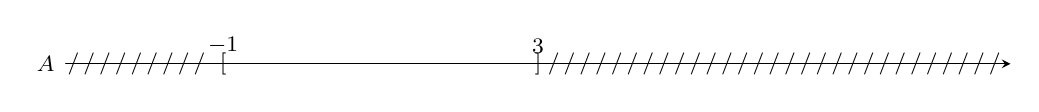
\begin{tikzpicture}[font=\footnotesize, line cap=round, line join = round, >=stealth]
\draw[-stealth] (-3,0)node[left=0.5]{$A$}--(-1,0)node[above=0.2]{$-1$}node {$[$}--(3,0)node[above=0.2]{$3$}node{$]$}--(9,0);

\foreach \x in {-2.9,-2.7,...,-1.2}
\draw (\x ,0)node{$/$};
\foreach \y in {3.2,3.4,...,8.8}
\draw (\y ,0)node{$/$};
\end{tikzpicture}\\
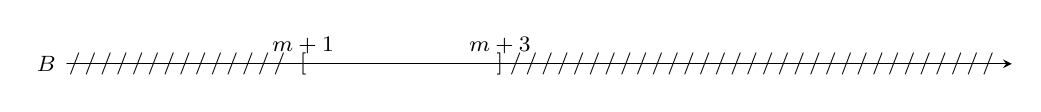
\begin{tikzpicture}[font=\footnotesize, line cap=round, line join = round, >=stealth]
\draw[-stealth] (-3,0)node[left=0.5]{$B$}--(0,0)node[above=0.2]{$m+1$}node {$[$}--(2.5,0)node[above=0.2]{$m+3$}node{$]$}--(9,0);

\foreach \x in {-2.9,-2.7,...,-0.2}
\draw (\x ,0)node{$/$};
\foreach \y in {2.7,2.9,...,8.8}
\draw (\y ,0)node{$/$};
\end{tikzpicture}
\end{center}
Ta có 	$ B \subset A \Leftrightarrow -1\le m+1<m+3 \le3 \Leftrightarrow -2 \le m\le 0\Leftrightarrow m\in \left[ -2;0\right] $.
}
\end{ex}

\begin{ex}%[0K1K2-2]
Cho các tập hợp khác rỗng $ A=[2m+1;m+4]$ và  $ B=(-\infty;-1]\cup (5;+\infty)$. Tìm tất cả các giá trị thực của $ m $ để $ A\cap B=\varnothing $.
\choice
{$ \hoac{&m\leq -1\\&m>1} $}
{$ -1<m\leq 1$}
{$ 1<m<3 $}
{\True $ \hoac{&1<m\leq 3\\&m\leq -1} $}
\loigiai{
Ta có 	$ A\cap B=\varnothing \Leftrightarrow\heva{&2m+1\leq m+4\\&\hoac{&2m+1\leq -1\\&m+4>5}}\Leftrightarrow\heva{&m\leq 3\\&\hoac{&m\leq -1\\&m>1}}\Leftrightarrow\hoac{&1<m\leq 3\\&m\leq -1.}$
}
\end{ex}

\begin{ex}%[0K1K2-2]
Cho hai tập hợp $A=\left\{ 1;3 \right\}$, $B=\left\{ x\in \mathbb{R}|x^2-mx+m-1=0 \right\}$. Với giá trị nào của $m$ thì $A\setminus B=\left\{ 3 \right\}$?
\choice
{ $m\ne 2$}
{ $m=4$}
{\True $m\ne 4$}
{ $m=2$}
\loigiai{
Ta có\\ $x^2-mx+m-1=0\Leftrightarrow \left( x-1 \right)\left( x+1-m \right)=0\Leftrightarrow \left[ \begin{aligned}
& x=1 \\
& x=m-1 .
\end{aligned} \right.$\\
Suy ra $B=\left\{ 1;m-1 \right\}$.\\
Khi đó, $A\setminus B=\left\{ 3 \right\}\Leftrightarrow m-1\ne 3\Leftrightarrow m\ne 4$.}
\end{ex}

\begin{ex}%[0K1K2-2]
Cho tập $A=\left\{ x \in \mathbb{Z} \mid \dfrac{x^2}{2x+3} \in \mathbb{Z} \right\}$. Số tập con của $A$ là
\choice
{$32$}
{\True $64$}
{$16$}
{$8$}
\loigiai{
Ta có $\dfrac{4x^2}{2x+3}=\dfrac{4x^2-9+9}{2x+3}=2x-3+\dfrac{9}{2x+3}$.\\
Với $x \in \mathbb{Z}$, từ giả thiết $\dfrac{x^2}{2x+3} \in \mathbb{Z}$ ta suy ra $\dfrac{4x^2}{2x+3} \in \mathbb{Z}
\Leftrightarrow
\dfrac{9}{2x+3} \in \mathbb{Z}
$
\[\begin{aligned}
&\Leftrightarrow
(2x+3) \in \big\{1;-1;3;-3;9;-9\big\}\\
&\Leftrightarrow
x \in \big\{-1;-2;0;-3;3;-6\big\}.
\end{aligned}\]
Với các số $x$ tìm được ta có bảng kết quả tính $\dfrac{x^2}{2x+3}$ như sau
\begin{center}
\begin{tabular}{|c|c|c|c|c|c|c|}
\hline
$x$ & $-1$ & $-2$ & $0$ & $-3$ & $3$ & $-6$ \\
\hline
$\dfrac{x^2}{2x+3}$ & $1$ & $-4$ & $0$ & $-3$ & $1$ & $-4$ \\
\hline
\end{tabular}
\end{center}
Vậy $A=\big\{-1;-2;0;-3;3;-6\big\}$ và $n(A)=6$ nên số tập con của nó là $2^6=64$.
}
\end{ex}

\begin{ex} %[0K1K2-1]
Cho tập hợp $M = \left\{ {\left( {x;y} \right)|x,y \in \mathbb{Z} ;y = \dfrac{{2x + 4}}{{x - 3}}} \right\}$ . Tập  $ M $ có bao nhiêu phần tử?
\choice
{ $ 6 $ }
{\True $ 8 $ }
{ $ 10 $ }
{ $ 4 $ }
\loigiai{ Ta có $ M $ là tập nghiệm nguyên của phương trình
$ y=\dfrac{2x+4}{x-3}=2+\dfrac{10}{x-3}\in \mathbb{Z}\Leftrightarrow 10 \,\vdots\, (x-3) \Leftrightarrow x-3\in \{\pm 1;\pm 2;\pm 5; \pm 10 \} \Leftrightarrow
x\in \{-7;-2;1;2;4;5;8;13 \}
$. \\
Vậy phương trình có 8 nghiệm nguyên nên $ M $ có 8 phần tử.
}
\end{ex}

\begin{ex}%[0K1K1-2]
Trong các mệnh đề sau đây, mệnh đề nào có {\bf{mệnh đề đảo}} là đúng?
\choice
{Nếu  $ a $ và $ b $  cùng chia hết cho $ c $  thì $ a+b $  chia hết cho $ c $}
{Nếu hai tam giác bằng nhau thì diện tích bằng nhau}
{\True Nếu $ a $  chia hết cho  $ 3 $ thì $ a $  chia hết cho  $ 9 $}
{Nếu một số tận cùng bằng $ 0 $  thì số đó chia hết cho $ 5 $ }
\loigiai{
\begin{itemize}
\item Xét \lq\lq  Nếu  $ a $ và $ b $  cùng chia hết cho $ c $  thì $ a+b $  chia hết cho $ c $\rq\rq\\
Mệnh đề đảo là \lq\lq  Nếu $ a+b $  chia hết cho $ c $  thì  $ a $ và  $ b $ cùng chia hết cho $ c $\rq\rq\, là một mệnh đề sai.
\item Xét  \lq\lq  Nếu hai tam giác bằng nhau thì diện tích bằng nhau\rq\rq\, mệnh đề đảo là \lq\lq  Nếu hai tam giác có diện tích bằng nhau thì bằng nhau\rq\rq\, là một mệnh đề sai.
\item Xét \lq\lq  Nếu $ a $  chia hết cho  $ 3 $ thì $ a $  chia hết cho  $ 9 $\rq\rq\,mệnh đề đảo: \lq\lq  Nếu $ a $  chia hết cho $ 9 $  thì $ a $  chia hết cho  $ 3 $\rq\rq\, là một mệnh đề đúng.
\item Xét \lq\lq  Nếu một số tận cùng bằng $ 0 $  thì số đó chia hết cho $ 5 $ \rq\rq\, mệnh đề đảo: \lq\lq  Nếu một số chia hết cho $ 5 $ thì có số tận cùng bằng $ 0 $\rq\rq\, là mệnh đề sai vì có thể số tận cùng bằng $ 5 $.
\end{itemize}
}
\end{ex}

\begin{ex}%[0K1K1-2]
Trong các mệnh đề sau, có bao nhiêu mệnh đề đúng?\\
$P\colon$ \lq\lq  Với mọi số tự nhiên $ n $  và $ n^3 $  chia hết cho $3$ thì $ n $  chia hết cho $3$\rq\rq.\\
$Q\colon$ \lq\lq  $\exists n\in\mathbb{N}, (n^2+1)$ chia hết cho  $4$\rq\rq.\\
$K\colon$ \lq\lq  Cho $ a, b, c $  dương thỏa mãn  $ abc=1 $. Nếu $ a+b+c>\dfrac{1}{a}+\dfrac{1}{b}+\dfrac{1}{c} $  thì có một và chỉ một trong ba số $ a, b, c $  lớn hơn một\rq\rq.\\
$L\colon$ \lq\lq  Nếu phương trình bậc hai $ ax^2+bx+c=0 $  vô nghiệm thì $ a $ và $ c $ cùng dấu.\rq\rq
\choice
{$ 1 $}
{$ 2 $}
{\True $ 3 $}
{$ 4 $}
\loigiai{
\begin{enumerate}
\item Xét mệnh đề $ P $:\\
Giả sử $ n $ không chia hết cho $ 3 $ khi đó $ n=3k+1 $ hoặc $ n=3k+2 $, $ k\in\mathbb{N} $.\\
Với $ n=3k+1 $ ta có $ n^3=(3k+1)^3=27k^3+27k^2+9k+1 $ không chia hết cho $ 3 $ (mâu thuẫn).
Với $ n=3k+2 $ ta có $ n^3=(3k+2)^3=27k^3+54k^2+36k+4 $ không chia hết cho $ 3 $ (mâu thuẫn).\\
Do đó $ n $ chia hết cho $ 3 $. Suy ra mệnh đề $ P $ đúng.
\item Xét mệnh đề $ Q $: Với $ k\in\mathbb{N} $, ta có
\begin{itemize}
\item Khi $ n=4k\Rightarrow n^2+1=16k^2+1 $ không chia hết cho $ 4 $.
\item Khi $ n=4k+1\Rightarrow n^2+1=16k^2+8k+2 $ không chia hết cho $ 4 $.
\item Khi $ n=4k+2\Rightarrow n^2+1=16k^2+16k+5 $ không chia hết cho $ 4 $.
\item Khi $ n=4k+3\Rightarrow n^2+1=16k^2+24k+10 $ không chia hết cho $ 4 $.
\end{itemize}
$ \Rightarrow\forall n\in\mathbb{N}, n^2+1 $ không chia hết cho $ 4 $.\\
Do đó mệnh đề $ Q $ sai.
\item Xét mệnh đề $ K $: Giả sử ngược lại, khi đó ta có các trường hợp sau\\
TH1. Với ba số đều lớn hơn $1$ hoặc ba số đều nhỏ hơn $1$ thì mâu thuẫn với giả thiết.\\
TH2. Với hai trong ba số lớn hơn $1$, không mất tính tổng quát giả sử   $ a>1 $, $ b>1 $.\\
Vì $ abc=1 $ nên $ c<1 $ do đó
$(a-1)(b-1)(c-1)<0 \Leftrightarrow abc+a+b+c-ab-bc-ca-1<0\\
\Leftrightarrow a+b+c<ab+bc+ca\Leftrightarrow a+b+c<\dfrac{1}{a}+\dfrac{1}{b}+\dfrac{1}{c} \text{(mâu thuẫn)}$.\\
Thừ với $ a=b=c=1 $ ta có $ a+b+c=\dfrac{1}{a}+\dfrac{1}{b}+\dfrac{1}{c}=3 $ (không thỏa đề bài).\\
Vậy chỉ có một và chỉ một trong ba số $ a $, $ b $, $ c $  lớn hơn $ 1 $ suy ra mệnh đề $K$ đúng.
\item Xét mệnh đề $ L$: Giả sử phương trình vô nghiệm và $ a c\leq 0 $.\\
Suy ra $ \Delta =b^2-4ac=b^2+4(-ac)\geq 0 $.\\
Suy ra phương trình có hai nghiệm, điều này mâu thuẫn với giả thiết phương trình vô nghiệm.\\
Vậy phương trình vô nghiệm thì $ a $, $ c $  phải cùng dấu suy ra mệnh đề $L$ đúng.
\end{enumerate}
}
\end{ex}


\begin{ex}%[0K1G2-2]
Cho tập  $ A=(3;+\infty) $,  $ B=\{x\in\mathbb{R}, \vert x\vert>m\} $. Có bao nhiêu giá trị nguyên của tham số $ m\in[-20;20] $  để tập hợp $ (A\backslash B)\cap \mathbb{Z} $  có không quá $10$ phần tử?
\choice
{$ 35 $}
{\True $ 34 $}
{$ 36 $}
{$ 11 $}
\loigiai{
Xét bất phương trình  $ \vert x\vert >m $.	$ \qquad(1) $
\begin{enumerate}[TH 1:]
\item $ m<0 $\\
Bất phương trình $(1)$ có tập nghiệm    $ T=\mathbb{R}\Rightarrow B= \mathbb{R}\Rightarrow A\backslash B=\varnothing\Rightarrow (A\backslash B)\cap \mathbb{Z}=\varnothing$.\\
Suy ra $ m<0 $  thoả mãn yêu cầu bài toán.
\item $ m\geq 0 $.\\
Bất phương trình $(1)\Leftrightarrow \hoac{&x>m\,\text{khi}\,x\geq 0\\&-x>m\,\text{khi}\,x<0}\Leftrightarrow\hoac{&x>m\\&x<-m\Rightarrow B=(-\infty;-m)\cup (m;+\infty)}$.
\begin{itemize}
\item Với $ m\leq 3\Rightarrow A\subset B\Rightarrow A\backslash B=\varnothing\Rightarrow (A\backslash B)\cap \mathbb{Z}=\varnothing $.\\
Suy ra $ 0\leq m\leq  3 $  thoả mãn yêu cầu bài toán.
\item Với $ m>3$, khi đó $ A\backslash B=(3;m] $.\\
Tập hợp $ (A\backslash B)\cap \mathbb{Z} $ có không quá $10$ phần tử khi và chỉ khi tập hợp $ A\backslash B $  có không quá $10$ phần tử là số nguyên $ \Leftrightarrow m<14 $.\\
Kết hợp điều kiện suy ra  $ 3<m<14 $ thoả mãn yêu cầu bài toán.\\
Kết hợp trường hợp $1$ và $2$ suy ra  $ m<14 $.\\
Mặt khác,  $ m\in\mathbb{Z}, -20\leq m\leq 20 $ nên có $34$ giá trị tham số $ m $  thỏa mãn bài toán.

\end{itemize}
\end{enumerate}
}
\end{ex}

\begin{ex}%[0K1G2-3]
Cho hai tập hợp $A=\left\{ x\in \mathbb{N}|x^2-4x-5=0 \right\}$, $B=\left\{ x\in \mathbb{R}|\left( x-1 \right)\left( {x^2}-4 \right)=0 \right\}$. Tập hợp $A\cup B$ bằng
\choice
{ $\left\{ 1;2;-2 \right\}$}
{ $\left\{ -1;5;1;2;-2 \right\}$}
{ $\left\{ 5;1 \right\}$}
{\True $\left\{ 5;1;2;-2 \right\}$}
\loigiai{
Ta có\\ $x^2-4x-5=0\Leftrightarrow \left[ \begin{aligned}
& x=-1\notin \mathbb{N} \\
& x=5\in \mathbb{N} \\
\end{aligned} \right.\Rightarrow A=\left\{ 5 \right\}$.\\
Ta có\\ $\left( x-1 \right)\left( {x^2}-4 \right)=0\Leftrightarrow \left[ \begin{aligned}
& x-1=0 \\
& {x^2}-4=0 \\
\end{aligned} \right.\Leftrightarrow \left[ \begin{aligned}
& x=1\in \mathbb{R} \\
& x=2\in \mathbb{R} \\
& x=-2\in \mathbb{R} \\
\end{aligned} \right.\Rightarrow B=\left\{ 1;2;-2 \right\}$.\\
Khi đó $A\cup B=\left\{ 5;1;2;-2 \right\}$.}
\end{ex}

\begin{ex} %[0K1G2-2]
Cho tập $A=( 0; +\infty )$ và $B=\left\{  x\in \mathbb{R} \bigg|  mx^2-4x+m-3=0 \right\}$, $m$ là tham số. Có bao nhiêu giá trị của $m$ để $B$ có đúng hai tập con và $B\subset A$?
\choice
{ $0$}
{ $2$}
{ $4$}
{ \True $1$}
\loigiai{
Để $B$ có đúng hai tập con( là $\varnothing $ và $B$) thì $B$ chỉ có một phần tử.\\
Xét phương trình $mx^2-4x+m-3=0$ $( 1 )$ có nghiệm duy nhất\\
Trường hợp 1: $m=0$, ta có $( 1 )\Leftrightarrow $ $x=-\dfrac{3}{4}\notin ( 0; +\infty )$.
Suy ra $m=0$ không thỏa đề bài.\\
Trường hợp 2: $m\ne 0$, ta có $( 1 )$ có nghiệm duy nhất
\[ {\Delta }'=0\Leftrightarrow {{( -2 )}^2}-m( m-3 )=0\Leftrightarrow \hoac{
&m=4 \\
&m=-1.}\]
Với $m=4$, ta có $( 1 )\Leftrightarrow 4x^2-4x+1=0\Leftrightarrow x=\dfrac{1}{2}\in ( 0;+\infty )$.\\
Với $m=-1$, ta có $( 1 )\Leftrightarrow -x^2-4x-4=0\Leftrightarrow x=-2\notin ( 0;+\infty )$.\\
Vậy có $1$ giá trị $m=4$ để $B$ có đúng hai tập con và $B\subset A$.
}
\end{ex}

\begin{ex} %[0K1G1-2]
Có bao nhiêu cặp số $ (x;y) $  sao cho cả ba mệnh đề  $ P,\, Q,\, R $ dưới đây đều đúng
$P:"2{x^2} - xy + 9 = 0",\,\,Q:"2{x^2} + {y^2} \le 81"$   và $R:"x \in \mathbb{Z}"$ ?
\choice
{ $ 3 $ }
{\True $ 2 $ }
{ $ 4 $ }
{ $ 5 $ }
\loigiai{
Bài toán tương đương với hệ phương trình
$
\heva{P:& 2{x^2} - xy + 9 = 0\\Q:& 2{x^2} + {y^2} \le 81\\R:& x \in \mathbb{Z}.}\,
$
Thế $ y=2x+\dfrac{9}{x} $ từ $ P $ vào $ Q $, ta được
\[
2{x^2} + \left (2x+\dfrac{9}{x}\right )^2 \le 81 \Leftrightarrow 6x^2+\dfrac{81}{x^2}\leq 81
\Rightarrow
\heva{6{x^2}\leq 81\\ \dfrac{81}{x^2}\leq 45
}
\Leftrightarrow \heva{x^2\leq \dfrac{81}{8}=7,5\\ x^2\geq \dfrac{81}{45}=1,8}.
\]
Vì $ x\in \mathbb{Z} $ nên $ x^2=4\Leftrightarrow x=\pm 2\Rightarrow y=\pm \dfrac{17}{2} $. Thử lại thoả hệ phương trình.\\
Vậy có tất cả 2 cặp số $ (x;y) $ thoả yêu cầu bài toán.
}
\end{ex}

\begin{ex}%[0K1G1-5]
Cho các mệnh đề sau
\begin{itemize}
\item $P$: ``$12500$ có tất cả $36$ ước số nguyên''.
\item $Q$: ``$\forall n \in \mathbb{N} \mid (n^5+9n) \;\vdots\; 5$ ''.
\item $R$: ``$\exists m \in \mathbb{Z} \mid x^2-4mx-2m-2=0 \text{ và } 2x^2+4mx-2m+1=0 \text{ có nghiệm chung}$''.
\end{itemize}
Có bao nhiêu mệnh đề đúng trong $3$ mệnh đề trên?
\choice
{$0$}
{$1$}
{$2$}
{\True $3$}
\loigiai{
\begin{itemize}
\item Ta có $12500=2^2 \cdot 5^5$ nên có số các ước số nguyên là $2 \cdot 3 \cdot 6=36$. Vậy $P$ đúng.
\item $n^5+9n=(n^5-5n^3+4n)+(5n^3+4n)=\underbrace{(n-2)(n-1)n(n+1)(n+2)}_{\vdots\; 5}+\underbrace{5n^3+5n}_{\vdots\; 5}$ nên $Q$ đúng.
\item Giả sử phương trình $x^2-4mx-2m-2=0$ và $2x^2+4mx-2m+1=0$ có nghiệm chung.\\
Khi đó hệ phương trình  $\heva{&x^2-4mx-2m-2=0~~(1)\\&2x^2+4mx-2m+1=0}$ có nghiệm.\\
Ta có $\heva{&x^2-4mx-2m-2=0\\&2x^2+4mx-2m+1=0} \Leftrightarrow \heva{&2x^2-8mx-4m-4=0\\&2x^2+4mx-2m+1=0.}$\\
Trừ từng vế của hệ ta được $12mx+2m+5=0 \Rightarrow x=\dfrac{-2m-5}{12m}$\\
Thay lại (1): $\left( \dfrac{-2m-5}{12m} \right)^2-4m\dfrac{-2m-5}{12m}-2m-2=0$
\[\begin{aligned}
&\Leftrightarrow
(-2m-5)^2-4m\cdot12m(-2m-5)-(2m+2)(12m)^2=0
\end{aligned}\]
Phương trình bậc ba trên có nghiệm nên $R$ đúng.
\end{itemize}
}
\end{ex}

\begin{ex} %[0K1G2-5]
Lớp $10 A$ trường THPT Nam Lý có $15$ học sinh giỏi Toán, $12$ học sinh giỏi Lý, $10$ học sinh giỏi Hóa, $4$ học sinh giỏi đúng hai môn Toán và Lý, $3$ học sinh giỏi đúng hai môn Toán và Hóa, $2$ học sinh giỏi đúng hai môn Lý và Hóa, $1$ học sinh giỏi cả ba môn Toán, Lý, Hóa. Hỏi lớp $10 A$ có tất cả bao nhiêu học sinh giỏi ít nhất một trong ba môn Toán, Lý, Hóa?
\choice
{ $27$}
{ $37$}
{ $47$}
{ \True $29$}
\loigiai{
\begin{center}
\begin{tikzpicture}[font=\footnotesize, line join=round, line cap=round, >=stealth]
\tikzset{s/.style={draw=blue,rounded corners=1mm,rectangle}}
\def\a{3.5}
\def\b{0.55*\a}
\def\c{0.65*\a}
\def\e{0.5*\c}
\def\f{0.5*\c}
\def\g{0.4*\c}
\def\m{0.4*\a}
\def\n{0.25*\a}
%\fill[brown,draw=black,opacity=0.7](\a,0)arc(0:360:{\a} and {\b});
\fill[white,draw=black](60:{\a} and {\b})arc(60:450:{\c} and {\e})(1,-0.5)arc(0:360: {\f} and {\g})
(0,0)arc(0:360: {\m} and {\n});
\begin{scope}
\clip(1,-0.5)arc(0:360: {\f} and {\g});
\clip(0,0)arc(0:360: {\m} and {\n});
\fill[blue!50,draw=black](60:{\a} and {\b})arc(60:450:{\c} and {\e});
\end{scope}
\draw
(60:{\a} and {\b})--++(80:1)node[s,above]{Lý}(0,0)arc(0:135: {\m} and {\n})--++(150:1.5)node[s,above]{Toán}
(1,-0.5)arc(0:270: {\f} and {\g})--++(-90:1)node[s,below]{Hóa}

;
\path [name path =one](60:{\a} and {\b})arc(60:450:{\c} and {\e});
\path[name path =two](1,-0.5)arc(0:360: {\f} and {\g});
\path[name path =three](0,0)arc(0:360: {\m} and {\n});
\draw[name intersections ={of= one and two,by ={A,B}}](B)--++(-45:0.5)node[s,below right]{12};
\draw[name intersections ={of= one and three,by ={C,D}}](C)--++(110:1)node[s,above]{15};
\draw[name intersections ={of= two and three,by ={E,F}}](F)--++(-110:1)node[below,s]{10};
\path [red](C)++(-40:0.5)node{3}++(-35:0.9)node{1}(B)++(-150:1)node{6}(B)++(150:0.75)node{1}(C)++(0:2.5)node{7}(F)++(70:0.5)node{2}(C)++(-120:1)node{9};
\end{tikzpicture}
\end{center}
Nhìn vào biểu đồ, số học sinh giỏi ít nhất $1$ trong 3 môn là $9+7+6+3+1+1+2 = 29$.
} \end{ex}

\begin{ex} %[0K1G2-4]
Cho hai tập hợp $A=\left\{ x\in \mathbb{R}: \ | mx-3 |=mx-3 \right\}$ và $B=\left\{  x\in \mathbb{R}:\ x^2-4=0 \right\}$. Tìm tất cả các giá trị của tham số $m$để $B\backslash A=B$.
\choice
{ $-\dfrac{3}{2}\le m\le \dfrac{3}{2}$}
{ $m<\dfrac{3}{2}$}
{ \True $-\dfrac{3}{2}<m<\dfrac{3}{2}$}
{ $m\ge -\dfrac{3}{2}$}
\loigiai{Ta có $| mx-3 |=mx-3\Leftrightarrow mx-3\geq 0$ nên $A=\left\{ x\in \mathbb{R}: \ mx-3\geq 0 \right\}$.\\
Lại có $x^2-4=0\Leftrightarrow x=\pm 2$ nên $B=\left\{ -2;2 \right\}$.\\
Để $B\backslash A=B\Leftrightarrow B\cap A=\varnothing \Leftrightarrow \heva{
& -2\notin A \\
& 2\notin A \\
}\Leftrightarrow \heva{
& -2m<3 \\
& 2m<3 \\
}\Leftrightarrow \heva{
& m>-\dfrac{3}{2} \\
& m<\dfrac{3}{2} \\
}\Leftrightarrow -\dfrac{3}{2}<m<\dfrac{3}{2}$.
}
\end{ex}

\begin{ex}%[0K1G2-6]
Cho các tập $A=\left[-1;\,5 \right]$, $B=\left\{ x\in \mathbb{R}: \left| x \right|\le 2 \right\}$, $C=\left\{ x\in \mathbb{R}: x^2-9>0 \right\}$ và $D=\left[ m; 2m+1 \right]$. Tính tổng các giá trị của $m$ sao cho $\left( \left( A\cup B \right)\setminus C \right)\cap D$ là một đoạn có độ dài bằng 1.
\choice
{ $0$}
{ $1$}
{\True $2$}
{ $-1$}
\loigiai{
\begin{enumerate}[+)]
\item $x\in \mathbb{R}:\left| x \right|\le 2\Leftrightarrow -2\le x\le 2$. Suy ra $B=\left[ -2;\,2 \right]$ $\Rightarrow A\cup B=\left[-2;\,5 \right]$.
\item $x\in \mathbb{R}: x^2-9>0\Leftrightarrow \left( x-3 \right)\left( x+3 \right)>0\Leftrightarrow \left[ \begin{aligned}
& \left\{ \begin{aligned}
& x-3>0 \\
& x+3>0 \\
\end{aligned} \right. \\
& \left\{ \begin{aligned}
& x-3<0 \\
& x+3<0 \\
\end{aligned} \right. \\
\end{aligned} \right.\Leftrightarrow \left[ \begin{aligned}
& x>3 \\
& x<-3. \\
\end{aligned} \right.$\\
Suy ra $C=\left( -\infty ;\,-3 \right)\cup \left( 3;\,+\infty \right)$ $\Rightarrow \left( A\cup B \right)\setminus C=\left[ -2;\,3 \right]$.
\item  Vì $\left( A\cup B \right)\setminus C$ là một đoạn có độ dài bằng $5$ nên để $\left( \left( A\cup B \right)\setminus C \right)\cap D$ là một đoạn có độ dài bằng $1$ thì sẽ xảy ra các trường hợp sau:
\begin{itemize}
\item $-2\le m\le 3\le 2m+1\Leftrightarrow \left\{ \begin{aligned}
& -2\le m\le 3 \\
& m\ge 1 \\
\end{aligned} \right.\Leftrightarrow 1\le m\le 3$.\\
Khi đó: $\left( \left( A\cup B \right)\setminus C \right)\cap D=\left[ m;\,3 \right]$.
Đoạn có độ dài bằng $1$ khi và chỉ khi \[3-m=1\Leftrightarrow m=2 \text{(thoả mãn)}.\]
\item $m\le -2\le 2m+1\le 3\Leftrightarrow \left\{ \begin{aligned}
& m\le -2 \\
& -\dfrac{3}{2}\le m\le 1 \\
\end{aligned} \right.\Leftrightarrow m\in \varnothing $.
\item $-2\le m\le 2m+1\le 3\Leftrightarrow \left\{ \begin{aligned}
& m\ge -2 \\
& -1\le m\le 1 \\
\end{aligned} \right.\Leftrightarrow -1\le m\le 1$.\\
Khi đó: $\left( \left( A\cup B \right)\setminus C \right)\cap D=\left[ m;\,2m+1 \right]$.
Đoạn có độ dài bằng $1$ khi và chỉ khi \[2m+1-m=1\Leftrightarrow m=0 \text{(thoả mãn)}.\]
\end{itemize}
\end{enumerate}
Vậy tổng các giá trị $m$ thoả mãn bằng $2$.}
\end{ex}
\Closesolutionfile{ans}
